Některé vhodné případy použití byly definovány v~průběhu textu. V~této sekci se zaměřím na obecné příklady použití, respektive na modelování základních situací. Poté shrnu zajímavé případy použití, které světově významné firmy používající Cassandru prezentovaly na Cassandra Summitu 2013 v~Londýně, kterého jsem se zúčastnil. V~poslední části této kapitoly se budu věnovat případům využití, které jsem sám použil ve své praxi a nebo navrhoval v~analýzách projektů. 

\section{Obecné modelování}

\subsection{Jednoduché struktury s~nesloženým primárním klíčem (Statické tabulky)}

Pokud struktura dat nevyžaduje žádné složité operace a dotazy a vystačíme si s~modelem, kde klíč je tvořen jedním sloupcem (tedy například pouze nějaký hash), můžeme použít jednoduchou definici tabulky jako v~\ref{CQL1}. Z~této tabulky pak jednoduše data čteme i zapisujeme tak, jak jsme zvyklí z~klasického SQL.

\subsection{Struktury se složeným primárním klíčem (Dynamické tabulky)}

Dříve než popíšeme, jakým způsobem je možné vytvářet dynamické tabulky, je potřeba vysvětlit, jak Cassandra zachází se skládáním primárních klíčů

\subsubsection*{Složené klíče}
V~Cassandře můžeme skládat klíče na 2 části (ty mohou být tvořeny jedním sloupcem nebo opět složenými sloupci). První část klíče se nazývá \uv{Partition Key} a určuje, z~čeho se bude skládat interní primární klíč, tedy ten, co se hashuje a následně distribuuje po clusteru. Druhá část klíče se nazývá \uv{Clustering Key}, který automaticky na daných sloupcích vytváří index a řadí data dle těchto sloupců. Interně slouží tyto sloupce jako prefix v~názvech ostatních sloupců a fragmentujeme podle nich data uvnitř jedné řádky. 

\begin{lstlisting}[caption={Ukázka složených klíčů},label=CQL2]
CREATE TABLE Cats (
  block_id uuid,
  breed text,
  color text,
  short_hair boolean,
  PRIMARY KEY ((block_id, breed), color, short_hair)
);
\end{lstlisting}

Příklad \ref{CQL2} ukazuje, že Partition Key je složený ze sloupců \emph{block\_id} a  \emph{breed} a clustering sloupce jsou \emph{color} a \emph{short\_hair}. Cassandra uloží data, která mají stejný \emph{block\_id}, ale jiný \emph{breed}, na jiný uzel než data, která mají hodnoty těchto sloupců stejné.  


\subsubsection*{Časosběrné události 1}
Ideálním příkladem na ilustraci toho, jak se používají složené klíče (respektive implementace dynamických tabulek), tedy využití vlastnosti Cassandry, že v~Column family nemusí mít pevný formát sloupců, jsou časosběrné události. Ukládáme různé hodnoty v~čase na různých místech nebo pro různé uživatele. Ukázkový příklad sbírá data na meteorologických stanicích a ukládá aktuální teplotu pro daný čas.

\begin{lstlisting}[caption={Dynamická tabulka 1},label=CQL3]
CREATE TABLE temperature (
   weatherstation_id text,
   event_time timestamp,
   temperature text,
   PRIMARY KEY (weatherstation_id,event_time)
);
\end{lstlisting}

Jako primární klíč jsme zvolili id stanice, které bude tvořit také interní klíč pro Cassandru a čas události, což bude název sloupce, který bude mít jako hodnotu aktuální teplotu. Sloupce se interně budou automaticky řadit podle času. Interně tedy bude následující tabulka vypadat následovně: 

\begin{figure}[h]
\centering
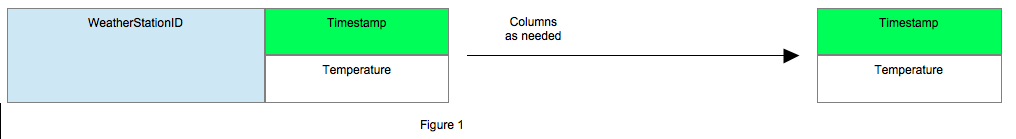
\includegraphics[scale=0.4]{images/timeseries1}
\caption{Interní reprezentace dat tabulky \ref{CQL3}}
\label{fig:timeseries1}
\end{figure}

Jak je z~obrázku \ref{timeseries1} patrné, tímto formátem využíváme zmíněnou výhodu o~odlišné struktuře řádek v~Column Family. Každá meteostanice má vlastní řádek a sloupce tvoří časové razítko, kdy byla naměřena daná hodnota. Časová razítka mohou být samozřejmě pro každou stanici jiná a tudíž bude mít i každá řádka odlišné sloupce. Takto můžeme data jednoduše vkládat a dotazovat se nad nimi. V~případě časosběrných událostí máme ovšem jednu nevýhodu. Jsme limitování maximálním počtem sloupců, kterých je sice asi 2 miliardy, ale pokud uvážíme, že bysme data měřili každou milisekundu, dojdou nám sloupce dřív než za měsíc.  

\subsubsection*{Časosběrné události 2}
U~předchozího řešení jsme narazili na problém, kdy nám mohou dojít sloupce pro danou řádku. Řešení tohoto problému je celkem jednoduché, použijeme při navrhování modelu vzor \uv{Rozdělení řádky}, kdy první část primárního klíče (Partition Key) složíme ze dvou sloupců stejně jako v~ukázce \ref{CQL2}.


\begin{lstlisting}[caption={Dynamická tabulka 2},label=CQL4]
CREATE TABLE temperature_by_day (
   weatherstation_id text,
   date text,
   event_time timestamp,
   temperature text,
   PRIMARY KEY ((weatherstation_id,date),event_time)
);
\end{lstlisting}

Tabulku jsme upravili tak, že jsme přidali sloupec \emph{datum}, který zároveň tvoří Partition Key. Data se budou ukládat pro každou stanici a každý den do samostatné řádky, čímž je limit 2 miliardy sloupců vyřešen, protože v~našem případě počítáme, že jedna stanice nebude denně provádět více než 2 miliardy měření. Interně to bude vypadat tak, že spojíme id stanice a datum, z~této hodnoty se vytvoří interní row key a ten rozhodne, na který uzel se data uloží. Schéma se změní následovně: 

\begin{figure}[h]
\centering
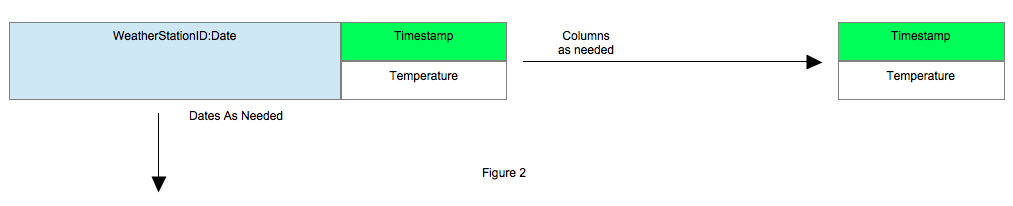
\includegraphics[scale=0.4]{images/timeseries2}
\caption{Interní reprezentace dat tabulky \ref{CQL4}}
\label{fig:timeseries1}
\end{figure}

Jak je vidět z~předchozího příkladu, návrh a struktura dat se musí opravdu dobře rozmyslet předem, případné chyby v~návrhu (např. opomenutí limitů) se poté řeší velice nepříjemně. Komplikovanější návrh nezabere implementačně moc času navíc a bude fungovat pořád.


\subsection{Mixování Statických a dynamických tabulek}
Cassandra nativně umožňuje i mixování předchozích vzorů. Například máme dynamický prvek \emph{tag}, který přiřazujeme k~uživateli, jehož ostatní sloupce jako jméno, adresa atd. jsou obyčejná statická tabulka. Cassandra takovýto návrh řeší nativně pomocí kolekcí. Kolekce jsou datový typ v~CQL, který umožňuje mít v~jednom sloupci více hodnot a pracovat s~nimi. Cassandra nabízí následující typy kolekcí:

\begin{itemize}
\item Set - ADT množina
\item List - ADT seznam
\item Map - ADT tabulka
\end{itemize}

Každý typ kolekce obsahuje odpovídající operace a chování, jaké se dá očekávat u~těchto abstraktních datových typů. Kolekce se dají použít kdykoliv, kdy chceme do statického modelu přidávat konečný (dopředu neznámý) počet malých hodnot. Kolekce mají následující omezení: 

\begin{itemize}
\item Maximální množství objektů v~kolekci je 64 000.
\item Maximální velikost objektu v~kolekci je 64Kb
\end{itemize}

\section{Jak Cassandru používají významné firmy a služby}

V~této sekci bych rád popsal několik reálných případu užití Cassandry ve všeobecně známých firmách či službách. Některé z~těchto případů užití byly demonstrovány na Cassandra Summit 2013, kterého jsem se v~rámci tvorby této práce zúčastnil a s~některými techniky daných firem jsem o~implementaci Cassandry v~jejich řešení hovořil. 

\subsection{Spotify a hudební seznamy}
Spotify je jedním z~největších hráčů na trhu online přehrávání hudby. Spotify však Cassandru nevyužívá k~ukládání informací o~skladbách či snad k~ukládání skladeb samotných, jak by se mohlo na první pohled zdát. Ve Spotify používají Cassandru k~ukládání seznamů skladeb. Takovýchto seznamů mají více než 1 miliardu a musejí řešit několik zádrhelů ohledně jejich kolaborativních úprav. Seznamy skladeb totiž mohou být editovatelné více uživateli nebo jedním uživatelem z~více míst a nebo dokonce je možné provádět jejich úpravy v~offline režimu. 

Ve Spotify si s~touto výzvou poradili výborně. Každý playlist je vlastně verzovaný objekt s~jednoduchými operacemi: \emph{MOV} posune skladbu z~nějakého místa na jiné, \emph{ADD} na vybrané místo skladbu vloží, \emph{DEL} vymaže skladbu ze seznamu. Každou takovouto operaci zaznamenávají se speciálním časovým razítkem a odkazem na předchůdce tohoto otce. Dále si v~jiné CF ukládají odkaz na takzvaný \emph{HEAD}, tedy poslední operaci. Díky souběžným změnám může být těchto hlaviček několik, což vede k~rozvětvení playlistu v~určitém bodě. Pomocí algoritmů operačních transformací dokáží z~libovolného místa seznam zreprodukovat a dokonce provést sjednocení rozdělených větví. Cassandra je tedy vhodná k~použití kdykoliv, kdy potřebujeme uložit velké množství jakkoliv verzovaných objektů. 

\subsection{Netflix}
Netflix patří mezi největší hráče na poli streamování video obsahu. Přestože se jedná v~principu o~podobnou službu jako Spotify, v~Netflixu využívají Cassandru pro ukládání úplně jiných dat. A~to téměř všech dat, které mají k~dispozici. Netflix má po celém světě přes 30 milionů aktivních uživatelů a do Cassandry ukládají informace o~uživatelích, metadata o~veškerém video obsahu nebo dokonce statistiky. Zajímavostí je, že Netflix nemá žádnou vlastní infrastrukturu a veškeré servery hostují přes službu Amazon AWS. Netflix je také jedním z~velkých přispěvatelů do zdrojových kódů Cassandry a to převážně právě do sekce věnující se nasazení a správě Cassandra clusteru na této službu od Amazonu. Tento případ užití by měl zviditelnit výhody ukládání plochých databázových struktur napříč několika datacentry po celém světě. 

\subsection{Ebay} 
Ebay je největší internetová aukční síň, která má desítky milionů uživatelů. Cassandru využívá na několik svých služeb. První z~nich je unikátní doporučovací systém. Každý uživatel prochází desítky položek při hledání určitého zboží a na základě toho, na které položky klikl nebo naopak neklikl, je mu doporučováno další zboží. Ebay ukládá veškeré tyto události formou grafu, který znázorňuje uživatele, nabízené zboží a vztahy mezi nimi. Díky tomuto systému může Ebay svým uživatelům nabízet stále přesnější výsledky. 

Ebay využívá Cassandru také na zpracovávání sociálních dat, jako jsou například zobrazení, přání a oblíbené položky. Tyto hodnoty pro jednotlivé produkty vždy napočítá pomocí MapReduce. 

Poslední případ, na který v~Ebayi Cassandru používají, jsou v~podstatě jakékoliv časosběrné události. Například:
\begin{itemize}
\item Mobilní notifikace jejich logování a sledování
\item Sledování dat pro následné odhalování podvodů
\item Analýza serverových logů a analytických dat
\end{itemize}

Využití Cassandry v~Ebayi ukazuje další stránky využitelnosti této databáze (například výše zmiňované časosběrné požadavky). Ebay považuje Cassandru za přínos hlavně z~hlediska škálovatelnosti a množství zápisů, které lze souběžně provádět. Ebay totiž za den provede do Cassandry přibližně 6 miliard zápisů.\cite{ebay} Ebay, kvůli plné integraci s~Hadoopem, navíc používá ve všech svých clusterech DataStax Enterprise, přes který provádí MapReduce. Schéma Ebay Cassandra clusteru vypadá přibližně následovně:

\begin{figure}[h]
\centering
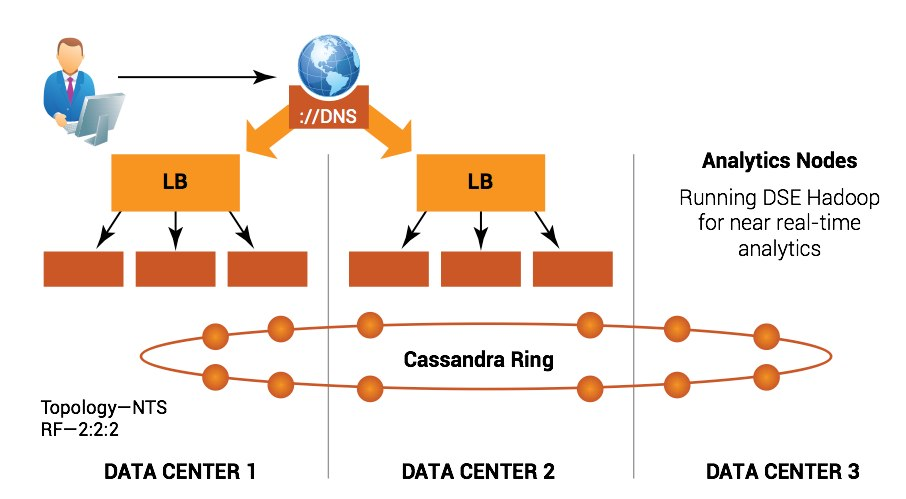
\includegraphics[scale=0.4]{images/ebay}
\caption{Ukázka sestaveni Cassandra clusteru v Ebay \cite{ebay}}
\label{fig:timeseries1}
\end{figure}

\subsection{Finn.no}
Finn.no je největší norský webový server. Týdně přivítá 3,5 milionu návštěvníků v~zemi, která má 5 milionů obyvatel. Jedná se o~inzertní portál, přes který lidé nabízejí či poptávají reality, pracovní pozice, věci na prodej, automobily, dovolené a služby. Na většinu z~těchto oblastí má Finn.no v~zemi \uv{monopol}. Tento inzertní server Cassandru opět využívá na několik způsobů. Prvním je ohodnocení každé nabídky, která přijde a její prověření, zda se nejedná o~podvod. V~případě podezření je taková nabídka přeposlána k~manuální kontrole. Dále Cassandru využívají na implementaci zpráv mezi uživateli, což je vlastně originální případ užití a důvod vzniku Cassandry kdysi v~kancelářích Facebooku. Cassandru zde využívají i na uchovávání uživatelovy historie hledání, kdy se uchovávají jednotlivé informace o~každém hledání a uživatel si může v~profilu prohlédnout, co hledal. V~tomto případě se návrháři rozhodli, že jim stačí uchovávat data pouze za posledních 6 měsíců, a proto využívají expirující sloupce, které po 6 měsících automaticky zmizí. Posledním případem využití je podobné sčítání zobrazení nebo přidání inzerátu do sledovaných jako na Ebay. Jednou za hodinu se spustí Hadoop Job, který pomocí MapReduce namapuje potřebné údaje, posčítá je a následně uloží zpět do databáze.

Zajímavostí na implementaci Finn.no je, že většina firem používá více menších strojů. Ve Finn.no mají pouze 6 uzlů s~velice výkonným hardwarem. Důvodem je lokalita dat, která pro ně má mnohem větší cenu než drobné blokující IO operace. 

\section{Ostatní navržené případy užití}

V~této sekci bych se na závěr kapitoly chtěl zaměřit na případy užití, se kterými jsem přišel do styku v~reálném prostředí nebo je teoreticky navrhoval pro nerealizované či věděcké projekty. 

\section{Analýza Access logů}
První z~těchto zajímavých případů užití se týká analýzy access logů. Dostal jsem za úkol navrhnout řešení, které by umožnilo velké nadnárodní společnosti s~pobočkami po celém světě a více než 20 000 zaměstnanci monitorovat, jaké weby její zaměstnanci navštěvují v~pracovní době. Na základě těchto dat poté tvořit grafy a reporty pro konkrétní uživatele nebo oddělení. Součástí analýzy řešení byl i prototyp vybraného řešení. Seznam požadavků byl následující: 

\begin{itemize}
\item Možnost stahování či uploadu dat z~access logů do systému
\item Pro konkrétního uživatele či oddělení vyrobit report obsahující:
\begin{itemize}
\item Zobrazení dat za vybrané časové období (1 týden až 6 měsíců zpět) 
\item Zobrazení navštívených stránek s~absolutním číslem přístupů a procentuálním poměrem. 
\item Zohlednění příznaku firewallu o~statusu požadavku (OK, Podezřelý, Nepřípustný)  
\end{itemize}
\item Data uchovávat pouze po dobu 6 měsíců 
\item Data musí být přístupná ihned, avšak klidně s~denním zpožděním (logy se nestahují z~celého světa současně)
\end{itemize}

Po sběru požadavků jsem ihned identifikoval, že toto je přímo ukázkový příklad pro využití Cassandry. 

Tento případ užití jsem shledal natolik zajímavý a to jak z~hlediska možností implementace, praktického přínosu a významnosti, že jsem po domluvě s~vedoucím práce tento případ využití použil i v~praktické části a závěrečné části této práce, kde ho dopodrobna rozeberu.

\section{Obrázkové servery}
Dalším zajímavým případem využití, se kterým jsem se setkal, je i příklad užití, kde se čtení provádí mnohonásobně častěji než zápis. Takovým způsobem funguje obrázkový server. V~dnešní době mobilních zařižení je naprosto běžné, že potřebujeme mít obrázek v~několika velikostech. Vzhledem k~rostoucímu počtu různorodých zařízení vznikají potřeby pro nová a nová rozlišení. Na toto můžeme využít Cassandřinu vlastnost nepevného schématu. Pro každý obrázek uložíme originální velikost včetně metadat a při dotazu na něj příslušný obrázek vytáhneme z~databáze. Samozřejmě by celé řešení bylo vhodné doplnit o~nějakou vrstvu cachování. Tento use case je velice praktický a komplexní, jelikož závisí na ostatním nedatabázovém softwaru, a proto jsme se po konzultaci s~vedoucím práce rozhodli obrázek zařadit. Podobným způsobem uchovával své obrázky například Facebook, než napsal vlastní nízkoúrovňový systém na správu fotografií. 

\section{Sběr a vyhodnocení transakčních událostí}
V~maloobchodě je běžné zjišťovat oblíbenost produktů a hledat vazby mezi jednotlivými předměty a uživateli ukládáním všech transakcí a jejich následným přiřazováním ke konkrétním uživatelům (například v~e-shopu nebo pomocí věrnostní karty). Správnou manipulací s~daty jsme schopni vymodelovat například následující grafy:

\begin{itemize}
\item Uživatelé, co zakoupili produkt X, také zakoupili tyto produkty.
\item Graf uživatelů, kde hrany reprezentují vazbu alespoň jednoho společně zakoupeného předmětu. Ohodnocení hrany znamená počet takovýchto předmětů. 
\end{itemize} 
Předchozí grafy lze také upravovat změnou množiny předmětů a sledovat změny na základě určité skupiny předmětů. Takovéto grafy dokáží odhalit vazby mezi předměty, ale také vazby a podobnost mezi uživateli a předpovídat jejich další aktivitu. 
\newpage
\section{Hledání korelací}
Pokud máme dostatek dat, můžeme se mezi dvěma veličinami snažit o~hledání kovariance, respektive korelačního koeficientu. Veličinou myslíme hodnotu dat v~čase. Například každý den ukládáme, kolik jsme prodali kusů kterého zboží, jaká je teplota, jaký je aktuální kurz měny atd. Můžeme pak jednoduše hledat spojitosti například mezi počasím a počtem prodaného zboží nebo vztah 2 různých prodávaných artiklů mezi sebou. Pro obchodníky jsou poté tato data velice důležitá, protože jim pomáhají lépe pochopit myšlení svých zákazníků, předpovídat jejich chování a také lépe plánovat provoz svého podnikání. Tento případ užití si ve zjednodušené podobě popíšeme i v~následující kapitole. 

\section{Podpora v~plně distribuované síti}
Ing. Josef Gattermayer vede výzkumný projekt zabývající se plně distribuovaným systémem na rozesílání zpráv mezi uzly. Tento problém se zatím řeší pouze v~teoretické rovině a jedním z~problémů, který je potřeba vyřešit, je notifikování uzlů, které byly offline, že na ně někde čeká zpráva. 

V~tomto ohledu jsem se nechal inspirovat vlastností, kterou Cassandra používá při zapisování, a tou je konkrétně \uv{Hinted Handoff}, který byl popsán v~předchozích kapitolách. Tento návrh předpokládá, že cluster je (z~hlediska infrastruktury jednotlivých uzlů a služeb na nich běžících) nehomogenní. Návrh spočívá v~tom, že přestože by si všechny uzly byly rovny po stránce komunikační, některé uzly by byly zároveň uzly perzistentními, které by ukládaly informace například do Cassandry. Těmito perzistentními uzly by zpravidla měly být nějaké serverové stanice. U~ostatních komunikačních uzlů se nemusíme omezovat pouze na servery a můžeme počítat i se zařízeními, jako jsou mobilní telefony či přenosné počítače. Komunikační proces by v~případě neúspěšného doručení zprávy byl následující: 

\begin{enumerate}
\item Uzel A~vyšle zprávu pro uzel B
\item Uzel C zjistí nedoručitelnost, protože uzel B je nedostupný
\item Uzel C kontaktuje jeden z~perzistentních uzlů a zprávu do něj uloží s~určitou dobou platnosti. 
\end{enumerate}

Při změně stavu uzlu B zpět online se provedou následující operace:

\begin{enumerate}
\item Uzel B kontaktuje kterýkoliv perzistentní uzel s~dotazem, zdali pro něj má nějaké nedoručené zprávy
\item Perzistentní uzel pošle pro něj uchovanou zprávu uzlu B
\item Perzistentní uzel zašle zprávu o~doručení uzlu
A~\end{enumerate}


V~případě, že chceme striktně dodržovat distribuovanost informací, nebudeme na perzistentní server ukládat zprávy jako takové, ale budeme ukládat pouze takzvané hinty a operace budou probíhat následovně: 

\begin{enumerate}
\item Uzel A~vyšle zprávu pro uzel B
\item Uzel C zjistí nedoručitelnost, protože uzel B je offline
\item Uzel C zkontaktuje zpět uzel A~s~informací, že zprávu nelze odeslat
\item Uzel A~si zprávu uloží a zkontaktuje perzistentní server, aby uložil hint pro uzel B

\end{enumerate}

Při změně stavu uzlu B zpět online se provedou následující operace:

\begin{enumerate}
\item Uzel B kontaktuje kterýkoliv perzistentní uzel s~dotazem, zdali pro něj má nějaké nedoručené zprávy
\item Perzistentní uzel pošle uzlu B hint o~tom, že uzel A~pro něj má zprávu
\item Uzel C zašle uzlu A~požadavek na znovuposlání zprávy
\end{enumerate}


V~obou předchozích scénářích předpokládáme, že uzel B se stane nedostupným až po odeslání zprávy. Před odesláním zprávy si tuto informaci může zjistit uzel A~sám a provede tudíž operace, jako kdyby byl uzlem C, aniž by zprávu někam posílal. Ve druhé variantě je potřeba ošetřit problém cyklických hintů, pokud uzly budou navzájem střídavě nedostupné a pro jednu zprávu by mohlo být uloženo nekonečně mnoho hintů. Pro daný pár uzlů nám vždy stačí mít uložen právě jeden hint pro daný směr požadavku. Tento případ užití je pouze teoretický a měl by demonstrovat možnost využití distribuovaného systému, jako je Cassandra, v~jiných distribuovaných systémech jako úložiště nebo monitorovací prvek tohoto systému. 


\chapter{Popis implementace vybraných případů užití}
V~předchozí kapitole jsem popsal několik různých druhů užití Cassandry v~reálných podmínkách. Vzhledem k~zadání této práce jsem (po konzultaci s~jejím vedoucím) vybral několik jednoduchých a rozdílných případů, které budou sloužit jako podklady pro přípravu cvičení a laboratoří nově připravovaného předmětu na ČVUT.

\section{Testovací prostředí}
Součástí zadání bylo vypracovat tyto případy užití na školní infrastruktuře. Vzhledem ke komplikované instalaci a správě veškerého potřebného softwaru, bylo z~hlediska efektivity práce od této myšlenky upuštěno. Fakulta vlastní experimentální výpočetní cluster a Tomáš Bartoň, kterému bych tímto chtěl poděkovat, mi nabídl řešení, které se zprvu zdálo dostačující, ale vzhledem ke komplikacím jsme i od tohoto řešení museli upustit. Finální implementace tedy proběhla na clusteru vytvořeném z~virtuálních strojů na jednom fyzickém počítači pomoci XENu. Pro Ing. Gattermayera, který předmět připravuje, jsem připravil XEN obraz, díky kterému lze vytvořit nový uzel a spustit na něm Cassandru. Toto řešení se ukázalo i pro garanta předmětu jako nejvhodnější a nejjednodušší. 

\section{Implementace Access Log analyzéru}
Jak bylo zmíněno v~předchozí kapitole, dostal jsem za úkol vypracovat analýzu a prototyp řešení pro nadnárodní německou firmu zaměstnávající více než 20 000 lidí po celém světě. Tito lidé se z~firemní infrastruktury připojují do internetu a tato firma chce monitorovat návštěvnost stránek jednotlivých uživatelů a oddělení pro různá časová období, která však nejsou delší než 6 měsíců a na základě různých kriterií generovat online reporty. Tento zdánlivě jednoduchý problém v~sobě ve skutečnosti skrývá několik netriviálních úkolů. Především je to množství dat, které je potřeba zpracovat. Pokud bychom zpracovávali data sekvenčně, tak bychom museli procházet přibližně 1860 GB systémových logů, což bychom rozhodně v~žádné relační databázi nemohli provést v~rozumném čase. Data dostáváme inkrementálně každý den (vždy za předchozí den) a to v~několika dávkách z~různých serverů po celém světě. 


\subsection{Návrh řešení pro ukládání všech logů}
Rozhodl jsem se tedy, že budu data ukládat do tabulky v~Cassandře. Všechna data budu zapisovat s~atributem TTL tak, aby se za půl roku automaticky smazala. Strukturu tabulky jsem navrhl následovně: 

\begin{lstlisting}[caption={Návrh tabulky pro ukládání všech logů},label=LogTable]
CREATE TABLE accesslog_ks.logs ( 
user text,
date timestamp,
webpage text,
severity text,
PRIMARY KEY (user,date) 
);
\end{lstlisting}

Sloupec \emph{severity} znázorňuje \uv{nebezpečnost} dotazu, tak jak ji vyhodnotil proxy server. Tento údaj byl součástí analýzy a celý příklad značně komplikuje, jak bude vysvětleno níže. Jako primární klíč jsem zvolil návrhový vzor pro časosběrné údaje, tedy uživatele a časové razítko. Pro zjednodušení tohoto příkladu předpokládáme, že uživatel v~jednu vteřinu nepřistoupí na více webových stránek. V~reálném světě by bylo dobré do klíče přidat i webovou stránku či zpřesnit časové razítko až na milisekundy. 

\subsection{Naivní řešení}
Prvním řešením, jak získat data pro reporty, je dotazování se přímo nad tabulkou logů. Nápad by se mohl zdát naprosto špatný, ale opak je pravdou. Jak dokládá následující tabulka, pokud by nám šlo o~jedno konkrétní datum, je přístup do databáze velice rychlý i přes obrovské množství záznamů a prokazuje se, jak mocná Cassandra je. Čas nutný na přístup ke všem datům je na toto množství záznamů také výborný, avšak pro větší záznamy bychom již nedosahovali časů vhodných k~online reportu. Navíc v~této struktuře nemůžeme jednoduše třídit data a veškeré řazení a vyhodnocování bychom museli následně provádět v~kódu, což by bylo velice zdlouhavé a neefektivní. Nemluvě o~situaci, kdy bychom se dotazovali na různá oddělení a museli bychom provádět dotazů několik. Data v~tabulce neodpovídají reálnému provozu, všechny uzly se nachází na jednom ne příliš výkonném počítači s~jedním diskem, takže IO operace jsou velice limitované a následná komunikace s~testovacím prostředím probíhá přes lokální síť. Reálné hodnoty by byly mnohonásobně nižší, cílem je poukázat na rozdíl hodnot v~různých situacích.    

\begin{table}[h]
%\begin{tabularx}{\textwidth}{ |l|l|l|l||| }

    \begin{tabular}{|l|l|l|l|l|}
    \hline
    \begin{tabular}{@{}c@{}}Počet \\záznamů \end{tabular} &  \begin{tabular}{@{}c@{}}Přibližný počet \\záznamů na uživatele \end{tabular} &  Vše [ms] & 1/3 [ms] & 1 den [ms] \\ \hline
    1000          & 200                                  & 160                  & 40                 & 20               \\ \hline
    11000         & 2000                                 & 600                  & 300                & 60               \\ \hline
    111000        & 20000                                & 3887                 & 1243               & 70               \\ \hline
    \end{tabular}
    \caption {Měření dotazování nad tabulkou logů}
\end{table}

\subsection{MapReduce 1}
Samozřejmě existuje ještě lepší řešení, kterým je MapReduce. Data zredukujeme a uložíme do pomocné tabulky. Nejdříve projdeme schéma výsledné tabulky a následně si ukážeme mapovací a redukční funkci.

\begin{lstlisting}[caption={Tabulka pro ukládání reportů},label=ReportTable]
CREATE TABLE accesslog_ks.reports ( 
user text,
webpage text,
date timestamp,
severity text,
count int,
PRIMARY KEY ((user,severity),date,webpage) 
);
\end{lstlisting}

Formát tabulky je zde téměř stejný jako v~tabulce s~logy (až na pár výjimek). Sloupec \emph{date} nyní neoznačuje přesné časové razítko, nýbrž pouze označení data bez času. Navíc zde přibyl sloupec \emph{count}, který obsahuje informaci o~celkovém počtu navštívení dané webové stránky pro tento den. Velice důležité je zde složení primárního klíče, které určuje, jak se data budou ukládat a řadit uvnitř databáze. Důvody k~výše uvedené skladbě klíče jsou následující. 

Kvůli jednoznačnému určení potřebujeme, aby klíč obsahoval všechny výše zmíněné atributy. Abychom se mohli dotazovat na konkrétní uživatele, musí být uživatel Partition Key, respektive jeho první částí. Abychom se mohli dotazovat na všechny nebo pouze na vybrané úrovně závažnosti, musí být uvedeny jako druhá část partition klíče. Tato volba je přirozená, jelikož hodnota \emph{severity} nabývá konečného počtu předem známých hodnot, a proto nebudeme tolik fragmentovat. Kdybychom \emph{severity} a \emph{user} prohodili, mohli bychom se sice ptát na více uživatelů, ale pouze na jeden konkrétní stupeň závažnosti, což je vzhledem k~našemu zadaní nelogické a neoptimální.

Po partition klíči následují další části primárního klíče, jako je datum, protože podle něj se budou výsledky uvnitř partition řadit, což je přesně to, co chceme a navíc kdybychom \emph{date} a \emph{webpage} prohodili, museli bychom se dotazovat na konkrétní webovou stránku, abychom se vůbec mohli ptát na datum, což je vzhledem k~funkcím aplikace nesmyslné. Jak je vidět, pořadí sloupců tvořící primární klíč je velice důležité! Takto složený klíč je pro námi zadaný příklad jediné správné a optimální řešení.

\subsubsection{Mapovací funkce}
Mapovací funkce je v~tomto případě velice jednoduchá. Musíme vytvořit univerzální schéma klíče, abychom mohli sečíst návštěvy v~daný den. Proto potřebujeme datum \uv{normalizovat}. V~případě data nám stačí jej oříznout pouze na rok, měsíc a den. Čas požadavku nás nezajímá. Z~informací \emph{normalizované datum}, \emph{adresa}, \emph{uživatel} a \emph{úroveň závažnosti} vytvoříme klíč, ke kterému přiřadíme hodnotu 1, protože se jedná o~jednu návštěvu dané webové stránky v~jeden den konkrétním uživatelem. 

\subsubsection{Redukční funkce}
Redukční  Pro každý klíč provedeme sumu hodnot, tedy počtu navštívení a výsledek zapíšeme do výše uvedené tabulky s~výše popsaným primárním klíčem, který se rovná stejnému klíči, který jsme vytvořili v~mapperu. 

\subsection{MapReduce 2}
V~předchozím případě jsme viděli, jak napsat MapReduce job pomocí vlastního algoritmu, tedy nadefinování mapovací a redukční funkce. V~tomto případě to bylo relativně jednoduché a moc práce nám to nedalo. Přesto je potřeba napsat několik tříd a vše správně zkompilovat a poté spustit. V~druhém způsobu popíši, jak používat dotazovací jazyk Hive, který dotazy sám přeloží do MapReduce kódu, který spustí a vrátí výsledek. Tabulku na ukládání výsledků MapReduce jobů ponecháme stejnou jako v~prvním případě, výsledek je totiž stejný. V~jazyce Hive nám k~předchozímu výsledku stačí pouze takovýto dotaz:

\begin{lstlisting}[caption={Tabulka pro ukládání reportů},label=Hive1]
select 
to_date(cast(logs.date as bigint)) as trimdate,
logs.user,
logs.webpage,
logs.severity, 
count(*) as count
from logs 
group by logs.webpage, logs.severity, logs.user,
to_date(cast(logs.date as bigint));
\end{lstlisting}

Tento dotaz vypadá složitě, ale je to jednoduchý SQL dotaz, který je programátorům využívajícím SQL dobře srozumitelný. Jediná komplikovanější věc je funkce, která nám ořeže datum. Výsledkem tohoto dotazu jsou spočítané návštěvy stránek pro každý den pro všechny uživatele. Tento dotaz spustíme klasicky přes Hive JDBC konektor a jeho výsledky přes Cassandra JDBC konektor zapíšeme. Výsledek je stejný jako v~předchozím případě s~minimem psaní kódu, za cenu trochu delší doby běhu, která jde na vrub generování MapReduce jobu. 

Hive experimentálně podporuje i vkládání do Cassandry přes externí tabulku, kterou když vytvoříme, tak před dotaz \ref{hive1} vložíme příkaz \emph{INSERT INTO table}, kde \emph{table} je název naší externí tabulky. Kód pro vytvoření a namapování tabulky vypadá následovně: 

\begin{lstlisting}[caption={Vytvoření externí tabulky napojené na tabulku v~CQL},label=Hive2]
CREATE EXTERNAL TABLE hivereports (user string, webpage string,date timestamp, severity string, count int)
        STORED BY 'org.apache.hadoop.hive.cassandra.cql3.CqlStorageHandler'
        TBLPROPERTIES ( "cassandra.ks.name" = "accesslog_ks",
        "cassandra.cf.name" = "reports",
        "cassandra.ks.repfactor" = "2",
        "cassandra.ks.strategy" =
        "org.apache.cassandra.locator.SimpleStrategy");
    
ALTER TABLE hivereports SET TBLPROPERTIES ('cql3.output.query' = 'update accesslog_ks.reports set count = ? where user = ?  and webpage = ? and severity =?');
    
ALTER TABLE hivereports SET SERDEPROPERTIES ('cql3.update.columns' = 'user,webpage,date,severity,count');
\end{lstlisting}

Tento postup je ovšem vskutku experimentální a zatím nefunguje pro všechny případy, a proto se jeho užití zatím obecně nedoporučuje. V~případě napojení přes externí tabulku by nám tedy stačil jediný krátký dotaz a data by se nám uložila stejně jako v~prvním případě. Nevýhodou ovšem zůstává, že takto nemůžeme použít TTL funkci při zápisu do Cassandry.

\subsection{Optimalizace}
Jednou možnou optimalizací je omezení zadání na předdefinované celky času. Například jeden den zpět, minulý týden nebo minulý měsíc. Tedy, že výběr data nebude libovolný, čímž bychom snížili množství zápisů do tabulky reportů a výběr těchto dat by byl rychlejší. 

Druhou a poněkud zásadnější optimalizací je, že v~předchozích příkladech řadíme vždy z~celé množiny dat. Tomu můžeme předejít tím, že budeme MapReduce provádět pouze nad dnešními daty. Vzhledem k~pravidelnému inkrementálnímu přírůstku dat je tato optimalizace vhodná, protože nebudeme zbytečně pracovat s~daty, která už máme jednou vypočítaná. 

\subsection{Skupiny Oddělení}
Součástí zadání je, že uživatel může chtít zobrazit souhrnný report pro celé oddělení. V~současné variantě bychom museli pro každého uživatele z~oddělení udělat samostatný dotaz a výsledky spočítat. Takové řešení je samozřejmě neefektivní. Pomůžeme si jednoduchým trikem. Tabulku s~logy rozšíříme o~sloupec s~informací o~oddělení a vytvoříme druhý MapReduce nebo Hive dotaz, který nebude brát v~potaz sloupec s~uživatelem, ale ten o~oddělení a v~tabulce s~logy budeme mít záznamy i o~konkrétních odděleních. Nastane nám tím duplicita dat, která nám ovšem nevadí, jelikož je s~ohledem na ostatní řešení nejméně nevýhodná. 

\subsection{Statistiky}
V~případě, že by uživatelé chtěli vidět souhrnné statistiky, jako například počet navštívených stránek za včera (celkově) nebo nejoblíbenější stránky obecně, stačí pro každou z~těchto statistik vytvořit Hive dotaz. Přesně pro takové účely je totiž Hive ideální volbou.

\subsection{Zhodnocení případu užití}
Tento případ považuji z~hlediska praktického i názorného za velice užitečný a komplexní. Jedná se o~rozsáhlý případ poukazující na několik technologií. Z~hlediska nově připravovaného předmětu může být tento příklad použit na cvičeních věnujících se Cassandře, MapReduce, Hive. K~porozumění je potřeba znalost mechanismů z~přednášky. S~přihlédnutím k~rozsahu a komplexnosti tohoto případu jsme se s~vedoucím práce dohodli, že jej využijeme jako hlavní a do dopodrobna rozepsaný a ostatní případy budou popsány a neimplementovány v~menším detailu, aby došlo k~popsání základních principů použitých v~daném případu. 


\section{Obrázkový server}
Tento případ užití poukazuje na moderní přístup k~uchovávání obrázků a zároveň využití přístupu, kdy není pevně stanoveno schéma databáze. Přestože si vymodelujeme tabulku, která pevnou strukturu má, interně se přeloží do formátu bez pevného schématu. Opět se jedná o~reálný případ užití, který je používán a v~současné době uchovává 7 GB dat. 

V~dnešní době služby uchovávají velké množství obrázků a potřebují je zobrazit v~různých velikostech. Posílání univerzálního obrázku na všechny dotazy je nevhodné, stejně tak jako zmenšování obrázku na základě každého požadavku. Ukládání obrázků přímo do filesystému přináší řadu nevýhod. Musí se řešit záloha a distribuovanost celého FS, kontrola konkrétních souborů a hlavně limity. Systém, jako je Cassandra, je víc než vhodný na tuto práci. Celý obrázkový systém se bude skládat z~těchto částí:

\begin{itemize}
\item Vrstva cache na ukládání obrázků
\item Vrstva na úpravu obrázků 
\item Vrstva na ukládání obrázků a jejich čtení
\end{itemize} 


První dvě úrovně nás zajímají pouze teoreticky a záleží na konkrétních podmínkách, jaké řešení bude v~systému použito. Cachování obrázků je velice užitečné, protože chceme, aby u~často žádaných obrázků nikdy nedocházelo ke čtení z~disku. Vrstva na úpravu obrázků opět záleží na konkrétní volbě. V~našem případě postačí jakýkoliv software či knihovna, která umí obrázek zmenšit. 

Co je pro nás mnohem důležitější, je vrstva, která obrázky ukládá a čte. Když dostaneme požadavek na obrázek, podíváme se, zdali máme obrázek v~této velikosti uložený v~databázi. Pokud ano vrátíme obrázek, pokud ne, ale obrázek máme k~dispozici v~originální velikosti (tzn. obrázek evidujeme v~databázi), zmenšíme jej na požadovanou velikost a vrátíme jej uživateli. Následně obrázek uložíme zpět do databáze s~těmito rozměry a připravíme pro další použití. Pokud máme i cachovací vrstvu, je vhodné obrázek rovnou uložit i do cache. 

Schéma pro ukládání obrázků vypadá následovně. 

\begin{lstlisting}[caption={Tabulka pro ukládání obrázků v~různých velikostech},label=img1]
CREATE TABLE images ( 
  id text,
  width int,
  height int,
  data blob,
  metadata text, 
  PRIMARY KEY (id,width,height) 
);
\end{lstlisting}

Primárním klíčem je identifikátor včetně velikosti obrázku. Data se tedy budou rozdělovat podle tohoto identifikátoru (první část primárního klíče). Sloupec \emph{data} bude obsahovat serializovaný obrázek a sloupec metadata může obsahovat specifická metadata k~tomuto obrázku. Pokud bychom chtěli pro všechny obrázky se stejným id udržovat jedna metadata, bylo by lepší pro metadata založit samostatnou tabulku. V~případě, že každá velikost obrázku může mít jiná metadata, je tento návrh v~pořádku. 

V~aplikaci se poté jen dotážeme na obrázek v~dané velikosti a vyhodnotíme výsledky způsobem popsaným výše. 

\section{Hledání korelací mezi daty}
V~maloobchodě můžeme porovnávat například spojitost mezi prodejem dvou různých produktů nebo vliv počasí na prodeje. Jedná se o~časosběrnou událost, kdy za každý den ukládáme zisk za daný předmět (nebo počet prodaných kusů). Tyto data můžeme získávat pomocí MapReduce z~nějakého datasetu všech denních transakcí (například z~ERP). Tabulku si vymodelujeme například takto: 

\begin{lstlisting}[caption={Tabulka zisků z~prodeje předmětů v~daný den},label=corr1]
CREATE TABLE sales ( 
  productId int,
  soldUnits int,
  date timestamp,
  revenue double, 
  PRIMARY KEY (productId,date) 
);
\end{lstlisting}

Nyní se můžeme dotázat na data pro 2 různé produkty za určité časové období a pomocí matematické knihovny či tabulkového procesoru můžeme spočítat ku příkladu korelační koeficient, který nám určuje provázanost mezi daty. Tento postup určitě není nic nového a jedná se o~zaběhnutou praxi. Díky BigData se nám však naskýtá možnost pomocí například MapReduce zkoušet hledat korelaci napříč všemi různými daty automaticky. V~případě, že systém nalezne dobrý výsledek, oznámí nám to. Takto můžeme mezi svými daty hledat různé trendy. Je důležité si však uvědomit, že asociace dat neimplikuje kauzalitu. Na hledání trendů a korelací v~uživatelských datech existují i  specializované firmy, které jiným společnostem s~hledáním pomáhají. Hledání těchto informací totiž není triviální.

\section{Dotazování nad daty s~dvousměrnou vazbou}
Další možností případu užití je ukládání informací o~uskutečněných transakcích, kdy po každé transakci ukládáme, který uživatel si koupil jaký předmět. Tyto informace pro nás mají velkou informační hodnotu, protože nás může zajímat, kteří uživatelé si koupili konkrétní předmět nebo také jaké předměty si koupil konkrétní uživatel. V~malém elektronickém obchodě, který má pár desítek předmětů a pár set uživatelů, můžeme takovéto informace ukládat klasickým způsobem do relační databáze, která takovýto obnos dat bez problémů zvládne. V~případě, že máme několik desítek tisíc uživatelů a v~podstatě neomezený sortiment zboží a denně děláme několik stovek tisíc transakcí, dostáváme se do objemu dat, na který relační databáze nestačí a musíme použít nějaký NoSQL nástroj. Tento příklad užití by měl poukázat na to, že přestože je zadání velice triviální a jednoduše řešitelné pomocí relačních databází, tak při určitém objemu dat, se problém stává velice komplikovaným a musí se řešit pomocí komplexnějších nástrojů.

\begin{lstlisting}[caption={Vytvoření tabulky s~dvousměrnou vazbou pomocí indexu},label=CQL10]
CREATE TABLE itemstracking ( 
item text,
user text,
timestamp timestamp,
PRIMARY KEY (item)
);

CREATE INDEX userIndex ON itemstracking (user);
\end{lstlisting}

CQL neumí dotazování na sloupce mimo primární klíč. K~tomu Cassandra využívá sekundární indexy. Po přidání indexu může CQL dotaz obsahovat filtrování podle sloupce \emph{item} nebo \emph{user}. Přestože se nyní můžeme dotazovat díky indexu i na položky uživatele, v~dokumentaci Cassandry \cite{cassaindex} se dočteme, že používání indexů na sloupce s~velkou kardinalitou není vhodné vzhledem k~implementaci. Kdybychom měli velice omezený seznam uživatelů nebo předmětů, mohli bychom tabulku vymodelovat pomocí indexu. Toto řešení však v~našem případě není dostatečné. Dalším řešením je vytvořit si \uv{vlastní index} pomocí tabulky nebo si vytvořit další tabulku, kde budeme indexovat druhý parametr (tedy uživatele jako primární klíč). V~našem případě (při daném počtu sloupců) se jedná o~téměř totožná řešení. 

\begin{lstlisting}[caption={Vytvoření indexovací tabulky},label=CQL11]
CREATE TABLE userstrackingt ( 
item text,
user text,
timestamp timestamp,
PRIMARY KEY (user)
);
\end{lstlisting}

Nyní sice duplikujeme o~trochu více dat, než bychom duplikovali pomocí indexu (který indexuje data lokálně), ale nyní se můžeme jednoduše dotazovat na uživatele a předměty bez jakéhokoliv omezení na škálování a rozsah hodnot. 

\section{Ukládání Solr indexu do Cassandry}
Poslední demonstrovaný příklad ukáže použití vyhledávacího systému Solr, který byl popsán v~\ref{solr}. Tento systém indexuje data do lokálního souboru na disku. Fanoušci Cassandry společně s~firmou Datastax vytvořili modifikaci, díky níž se index ukládá přímo do Cassandry (lokálně) a data samotná se ukládají do Cassandry distribuovaně. Výhody tohoto řešení jsou zřejmé. Získáme distribuované vyhledávací řešení se všemi výhodami Cassandry. K~datům můžeme přistupovat pomocí Solr nebo CQL, což ponechává vysokou flexibilitu přístupu k~datům. Využití Solr je kompromisem mezi rychlostí Cassandry a analytickými schopnostmi Hadoopu. Patrně největšími benefity jsou automatické duplikování dat, automatické indexování dat vložených do Cassandry a také možnost zapisovat na kterýkoliv Solr uzel, čímž se minimalizuje problém úzkého hrdla při zápisu do Solr indexu. Příklad poukáže na základní vyhledávací vlastnosti Solr a jeho výhody oproti CQL.